\documentclass[9pt,a4paper]{article}
\usepackage{extsizes}

\usepackage[top=1.0cm, bottom=1.5cm, left=1.5cm, right=1.5cm]{geometry}
\usepackage{graphicx}
\usepackage{multicol}
\usepackage{booktabs}
\usepackage{tabularx}
\usepackage{caption}
\usepackage{subcaption}
\usepackage{enumitem}
\usepackage{hyperref}
\usepackage{titlesec}

% Compact spacing
\setlength{\parindent}{0pt}
\setlength{\parskip}{3pt}
\setlength{\columnsep}{12pt}
\titlespacing*{\section}{0pt}{4pt}{2pt}
\titleformat{\section}{\normalfont\bfseries\small}{\thesection.}{0.4em}{}

\pagestyle{empty}

\begin{document}

% ── Title ──────────────────────────────────────────────────────────
\begin{center}
{\large\bfseries Cross-Basin Generalization for Tropical Cyclone Forecasting\\using TropiCycloneNet}\\[3pt]
{\small Samuel Zhang, Loïc Bouxirot, Yasmin Akhmedova}\\
{\small\itshape Imperial College London, ELEC70127 ML for Tackling Climate Change}
\end{center}

\vspace{-2pt}
\hrule
\vspace{4pt}

% ── Two-column body ───────────────────────────────────────────────
\begin{multicols}{2}

\section*{Problem Context}

Tropical cyclone (TC) forecasting in data-scarce ocean basins is limited by small
training sets. The South Pacific (SP) contains 30 storms in the TropiCycloneNet
dataset, compared to 131 in the Western Pacific (WP), a ratio that makes it
impractical to train reliable models on SP alone~[1]. Transfer learning from
data-rich to data-scarce basins is a possible solution, and there is preliminary
evidence this works: Qu et al.\ (2025) fine-tuned a Western North Pacific-trained
transformer on the Eastern North Pacific and outperformed operational forecasting
systems~[2].

We focus on WP to SP as the transfer pair because it presents a structural
challenge beyond sample size. WP sits in the Northern Hemisphere and SP sits in
the Southern Hemisphere. The Coriolis force acts in opposite directions in each
hemisphere, so WP storms tend to move northwest/west while SP storms tend to move
southeast/west/southwest. A model trained on WP will therefore systematically
mispredict SP storm directions. However, the atmospheric physics governing TC
intensity, specifically sea-surface temperature and vertical wind shear, is shared
across both basins. DeMaria and Kaplan (1994) identify these as key intensity
predictors~[3], and our exploratory analysis confirms that their distributions
overlap substantially between WP and SP (Fig.~4).
\section*{Proposed Approach}

We evaluate five architectures on zero-shot WP to SP transfer, then fine-tune the best
performers. Each architecture offers a different reason to expect cross-basin generalisation:

\vspace{-2pt}
{\footnotesize
\begin{tabularx}{\linewidth}{@{}lX@{}}
\toprule
\textbf{Model} & \textbf{Why it might transfer} \\
\midrule
U-Net & Strong spatial feature extraction from 3D weather data (wind, temperature, pressure) and a well-established baseline for weather prediction \\
ResNet & Learns hierarchical features from gridded weather data with deep residual connections that help capture complex atmospheric patterns \\
FNO & Operates in frequency space so learned patterns are not tied to a specific grid or basin \\
PI-GAN & Designed to enforce physical conservation laws (vorticity, potential vorticity) that hold across hemispheres \\
Transformer & Fuses all three data modalities (1D, 3D, environmental) through cross-attention, allowing flexible reweighting across basins \\
\bottomrule
\end{tabularx}
}
\vspace{2pt}

\textit{Three-stage pipeline:}
\begin{enumerate}[nosep, leftmargin=1.2em, label=\arabic*.]
  \item \textit{Zero-shot}: Train each model on WP, remap directional labels to account for hemisphere differences, evaluate on SP with no fine-tuning.
  \item \textit{Fine-tune}: Adapt top-performing models on 10/25/50\% of SP data, measure how accuracy improves with increasing amounts of SP data.
  \item \textit{Extension}: Test whether the best models generalise to other data-scarce basins (NI, SI) without basin-specific retraining.
\end{enumerate}


\section*{Exploratory Data Analysis}

Four findings from our preliminary analysis support the proposed WP to SP transfer. The Basin Similarity Matrix in Fig.~1 shows that WP and SP have the lowest average Wasserstein distance across physical variables of any cross-hemisphere basin pair. Storm tracks in Fig.~2 show clear geographic separation and hemisphere differences in movement. Direction distributions in Fig.~3 confirm that WP and SP movement patterns are hemisphere-mirrored, with WP storms predominantly moving northwest and west while SP storms predominantly move southeast and west. This can be addressed by remapping directional labels before transfer. The vertical wind shear distributions in Fig.~4 overlap substantially between WP and SP, supporting the argument that intensity-related physics is shared across both basins.

\noindent
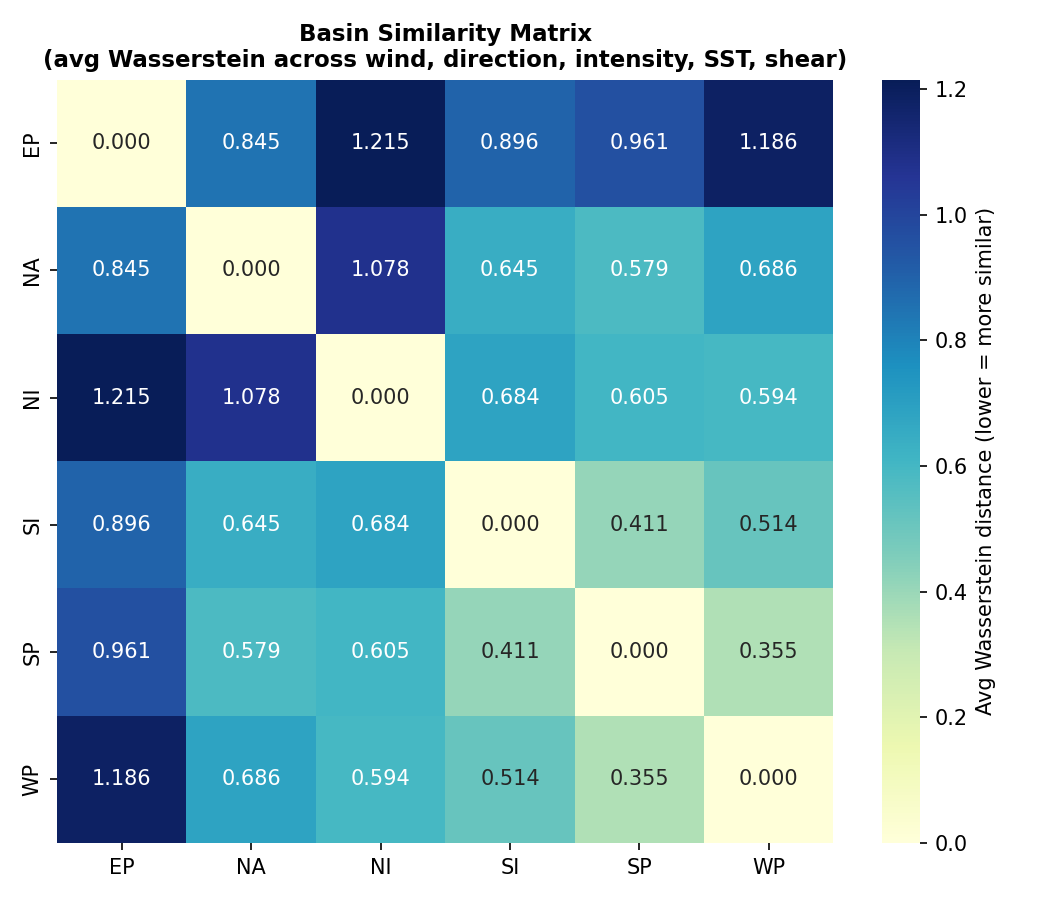
\includegraphics[width=\columnwidth]{../../figures/basin_similarity_matrix.png}
{\scriptsize\textbf{Fig.~1:} Average Wasserstein distance across wind, direction, intensity, SST and shear for all basin pairs. Lower is more similar.}


\noindent
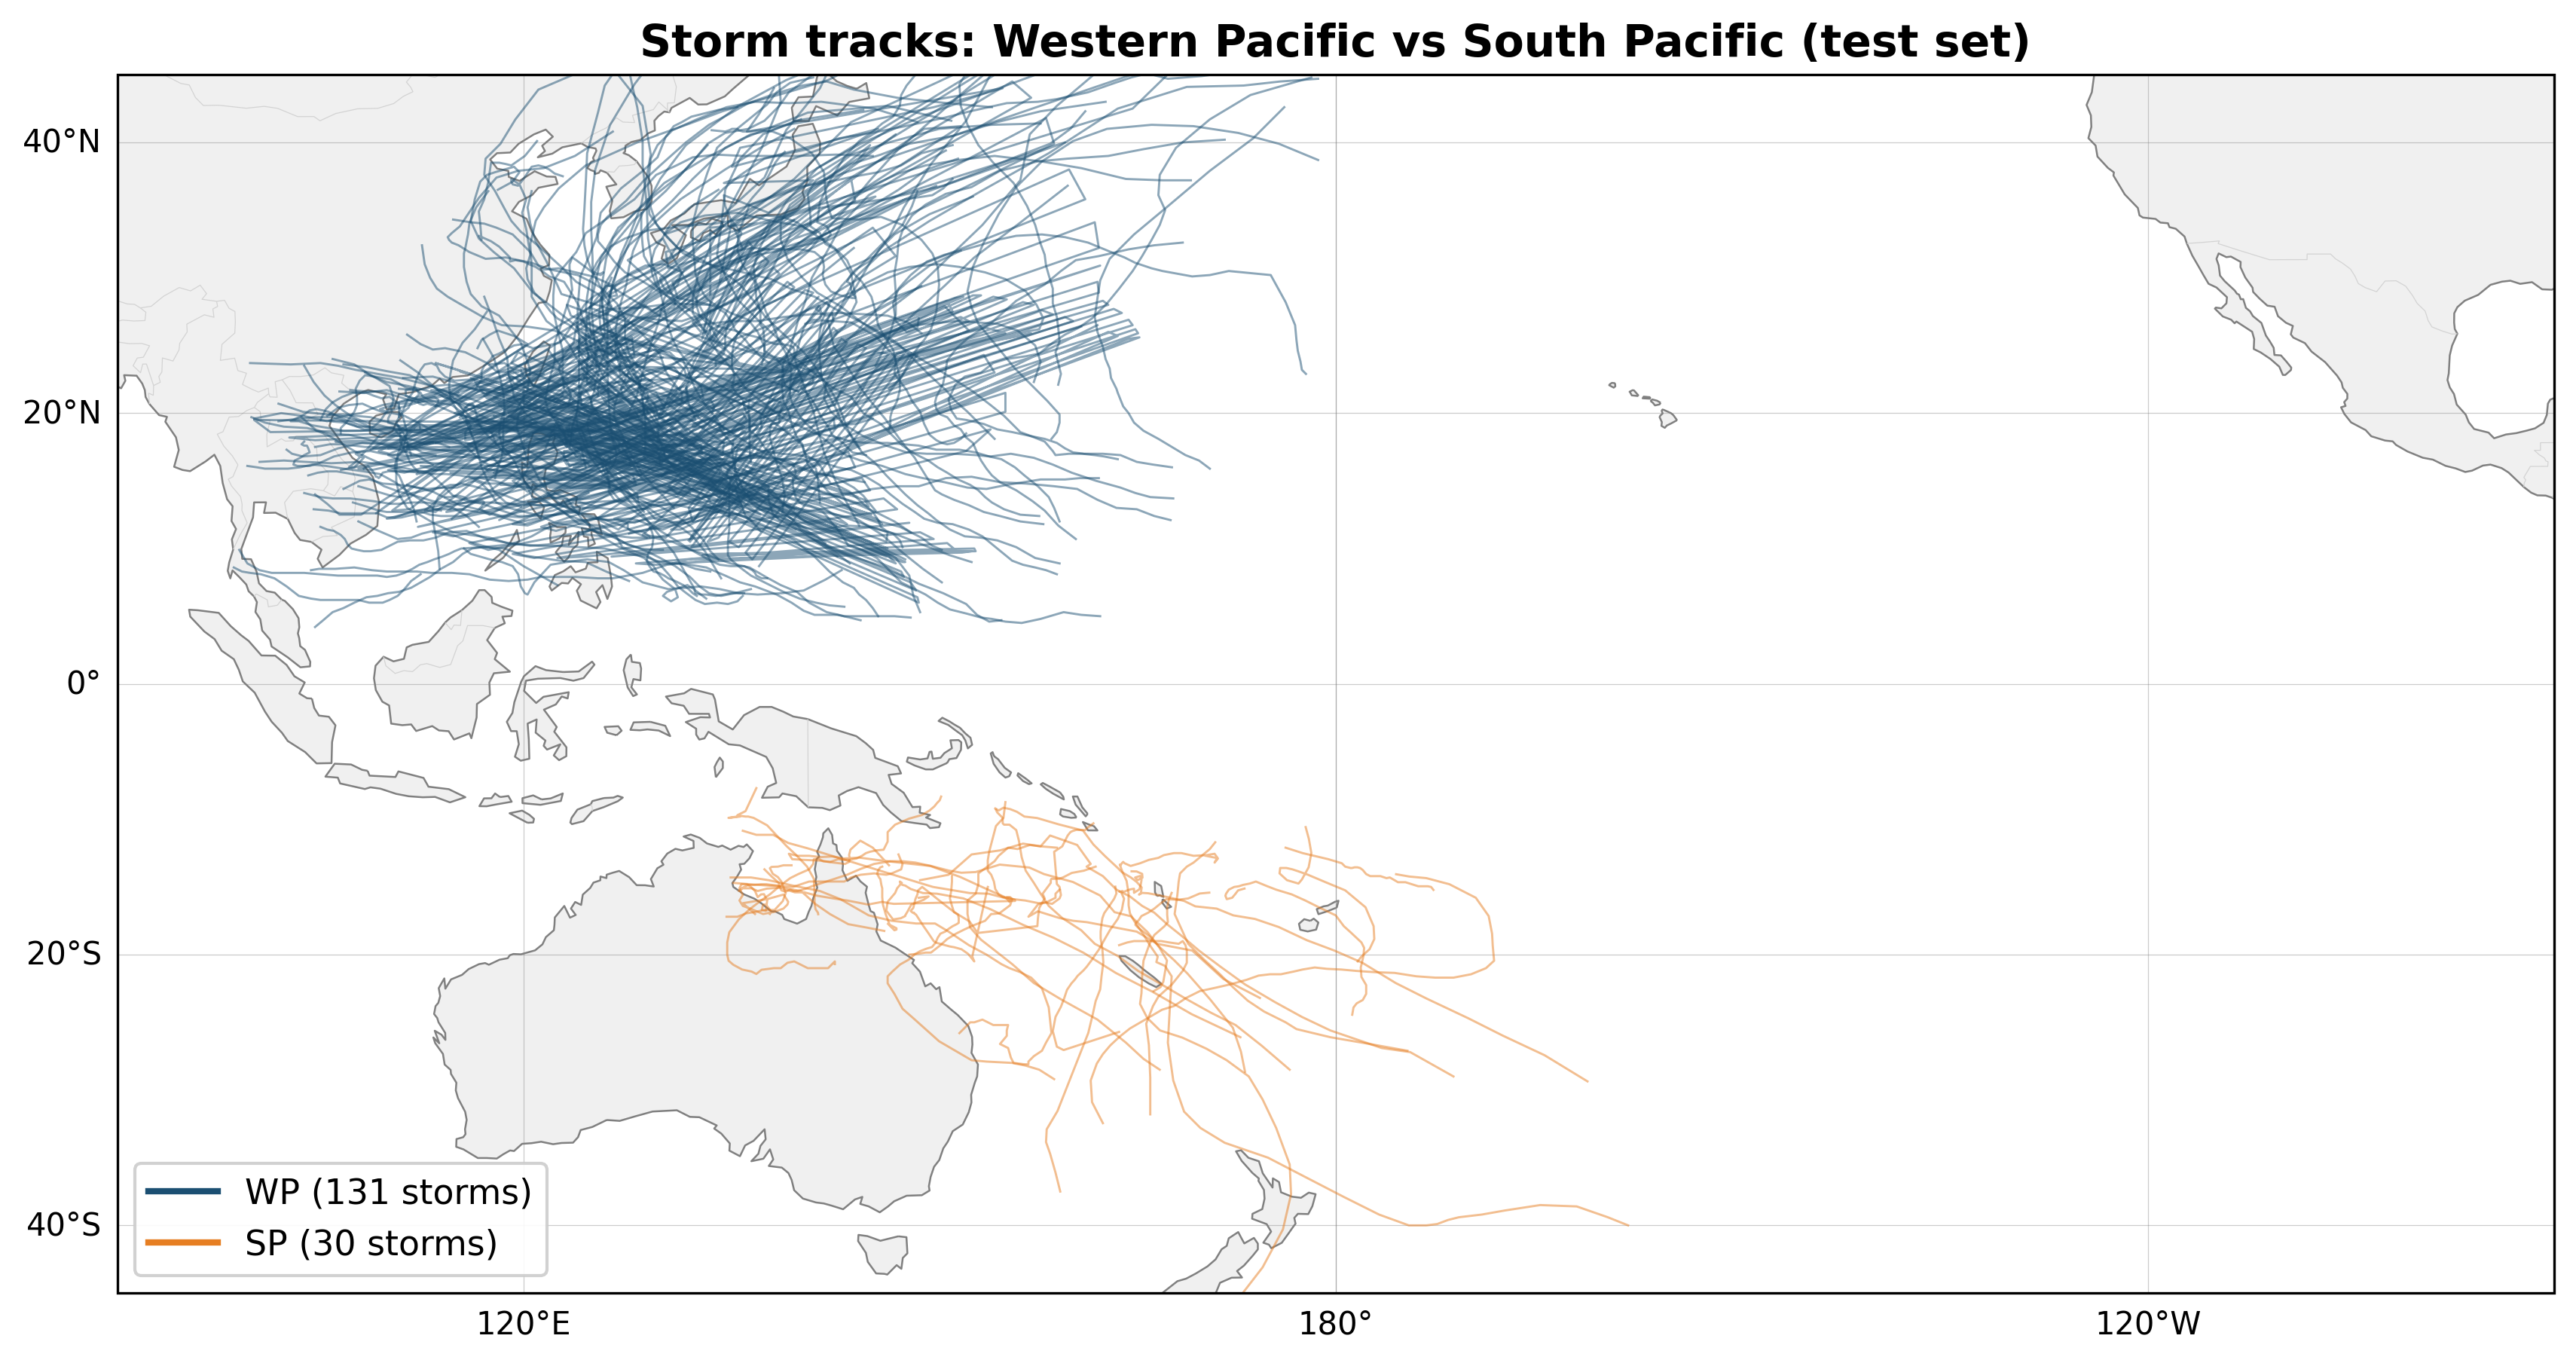
\includegraphics[width=\columnwidth]{../../figures/track_map.png}
{\scriptsize\textbf{Fig.~2:} WP (131 storms) and SP (30 storms) storm tracks.}

\noindent
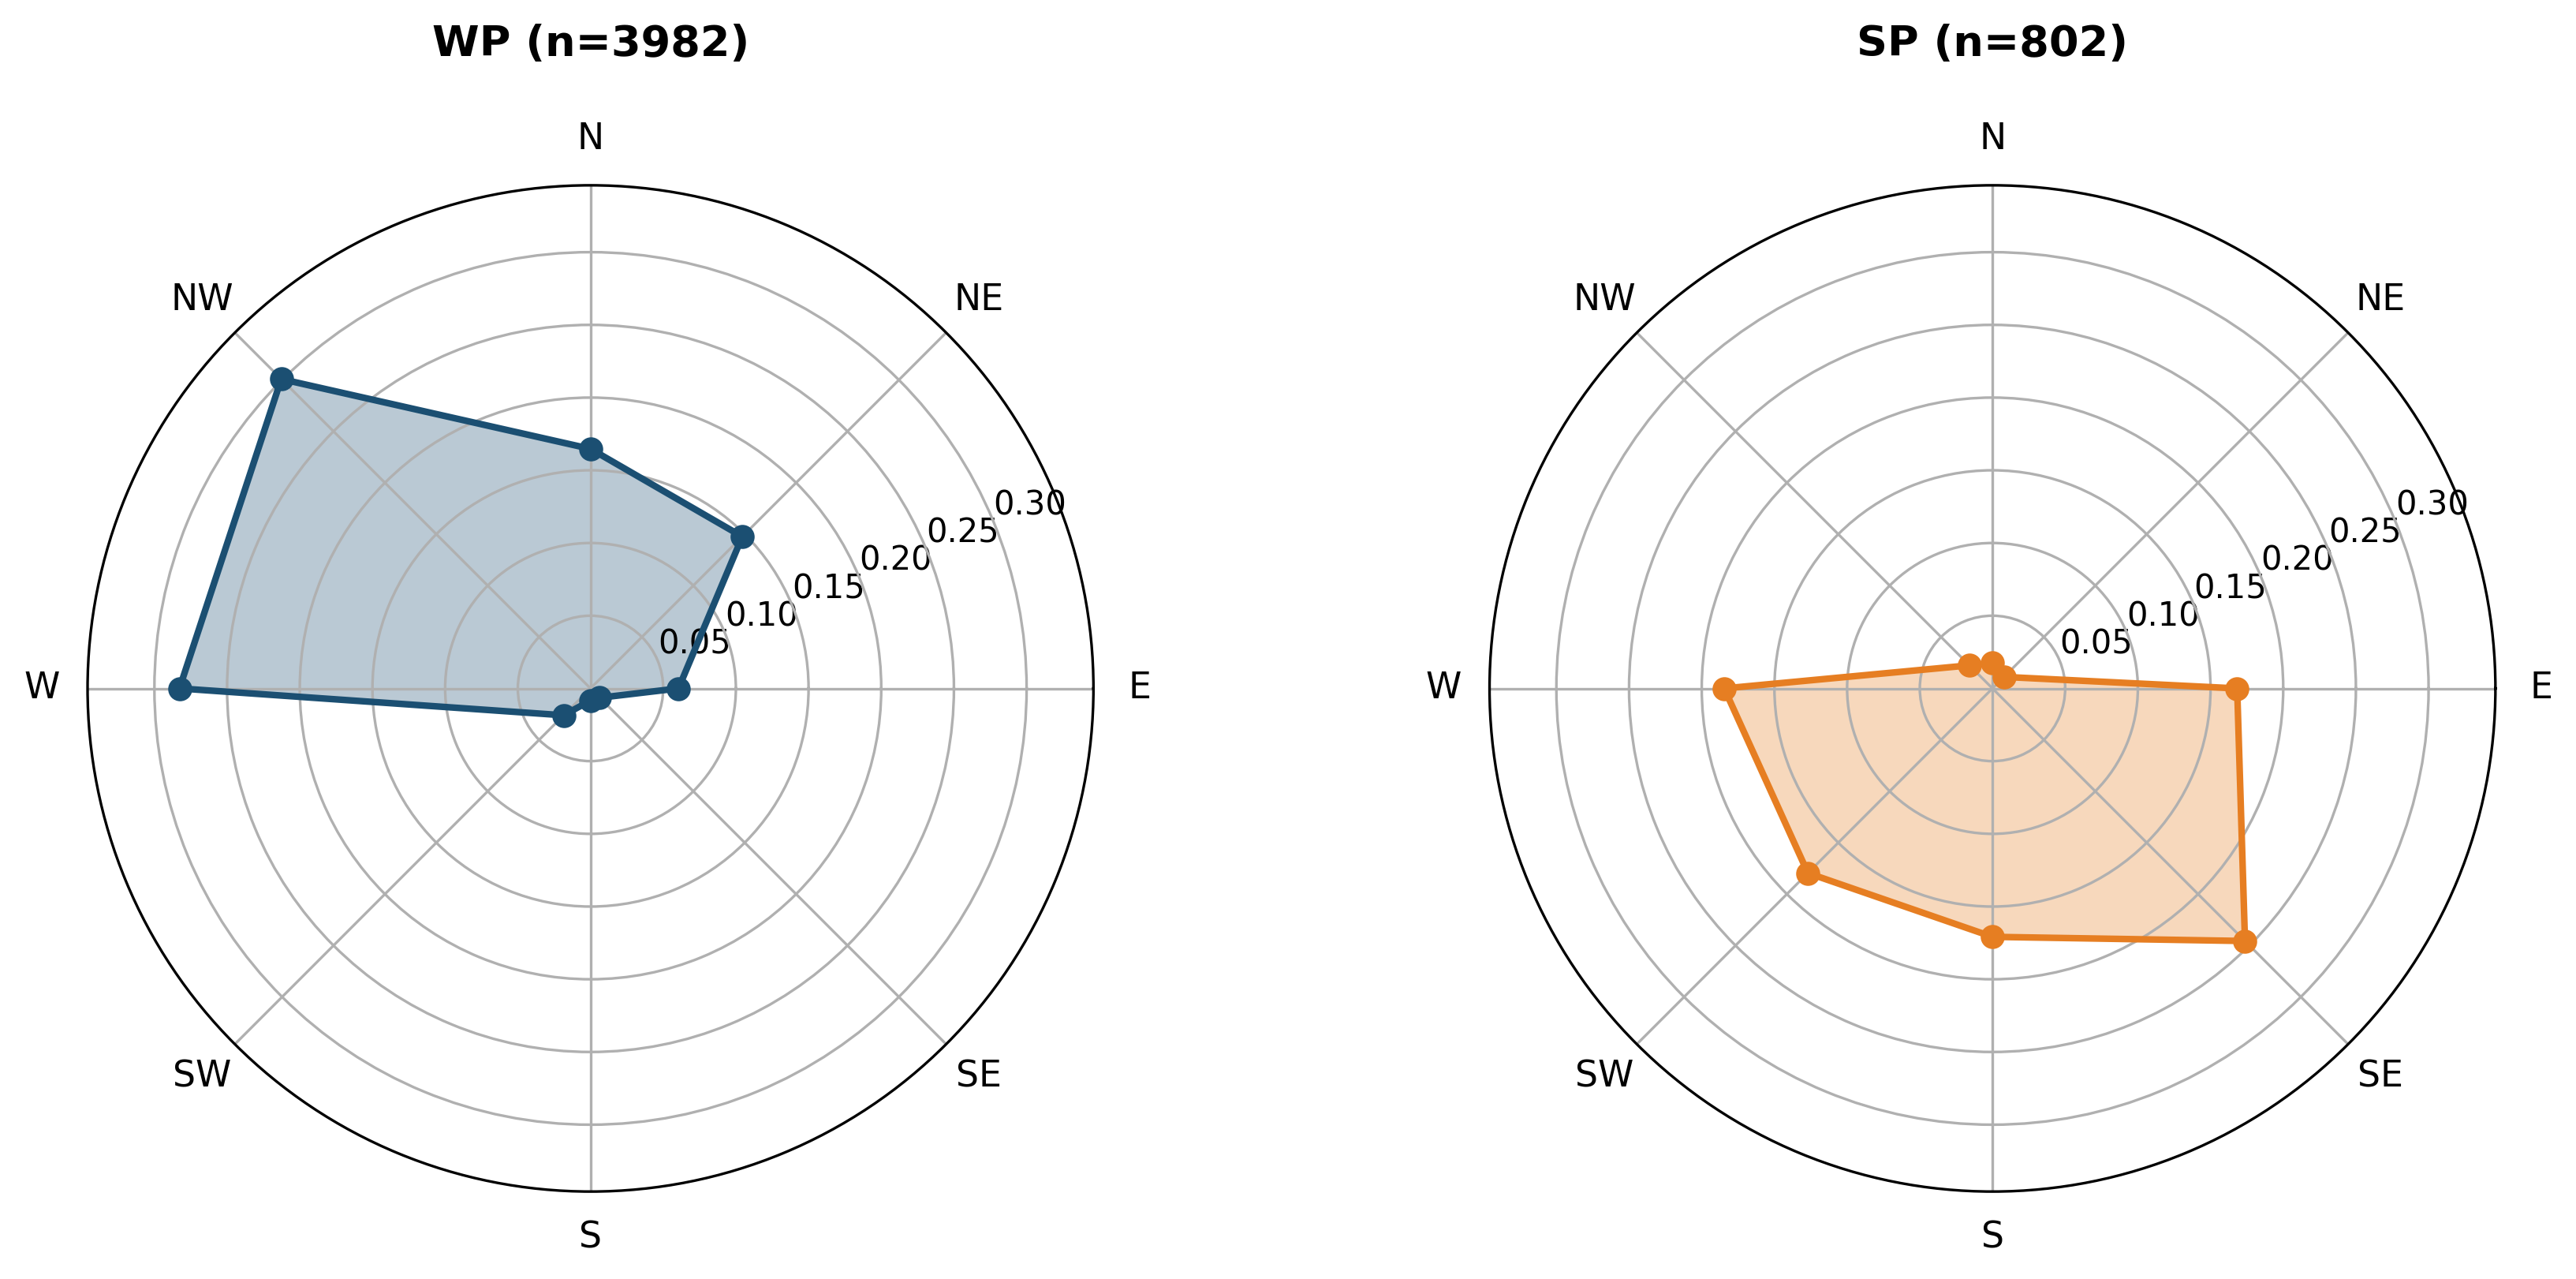
\includegraphics[width=\columnwidth]{../../figures/direction_distribution.png}
{\scriptsize\textbf{Fig.~3:} Direction polar roses for WP (n=3982) and SP (n=802).}

\noindent
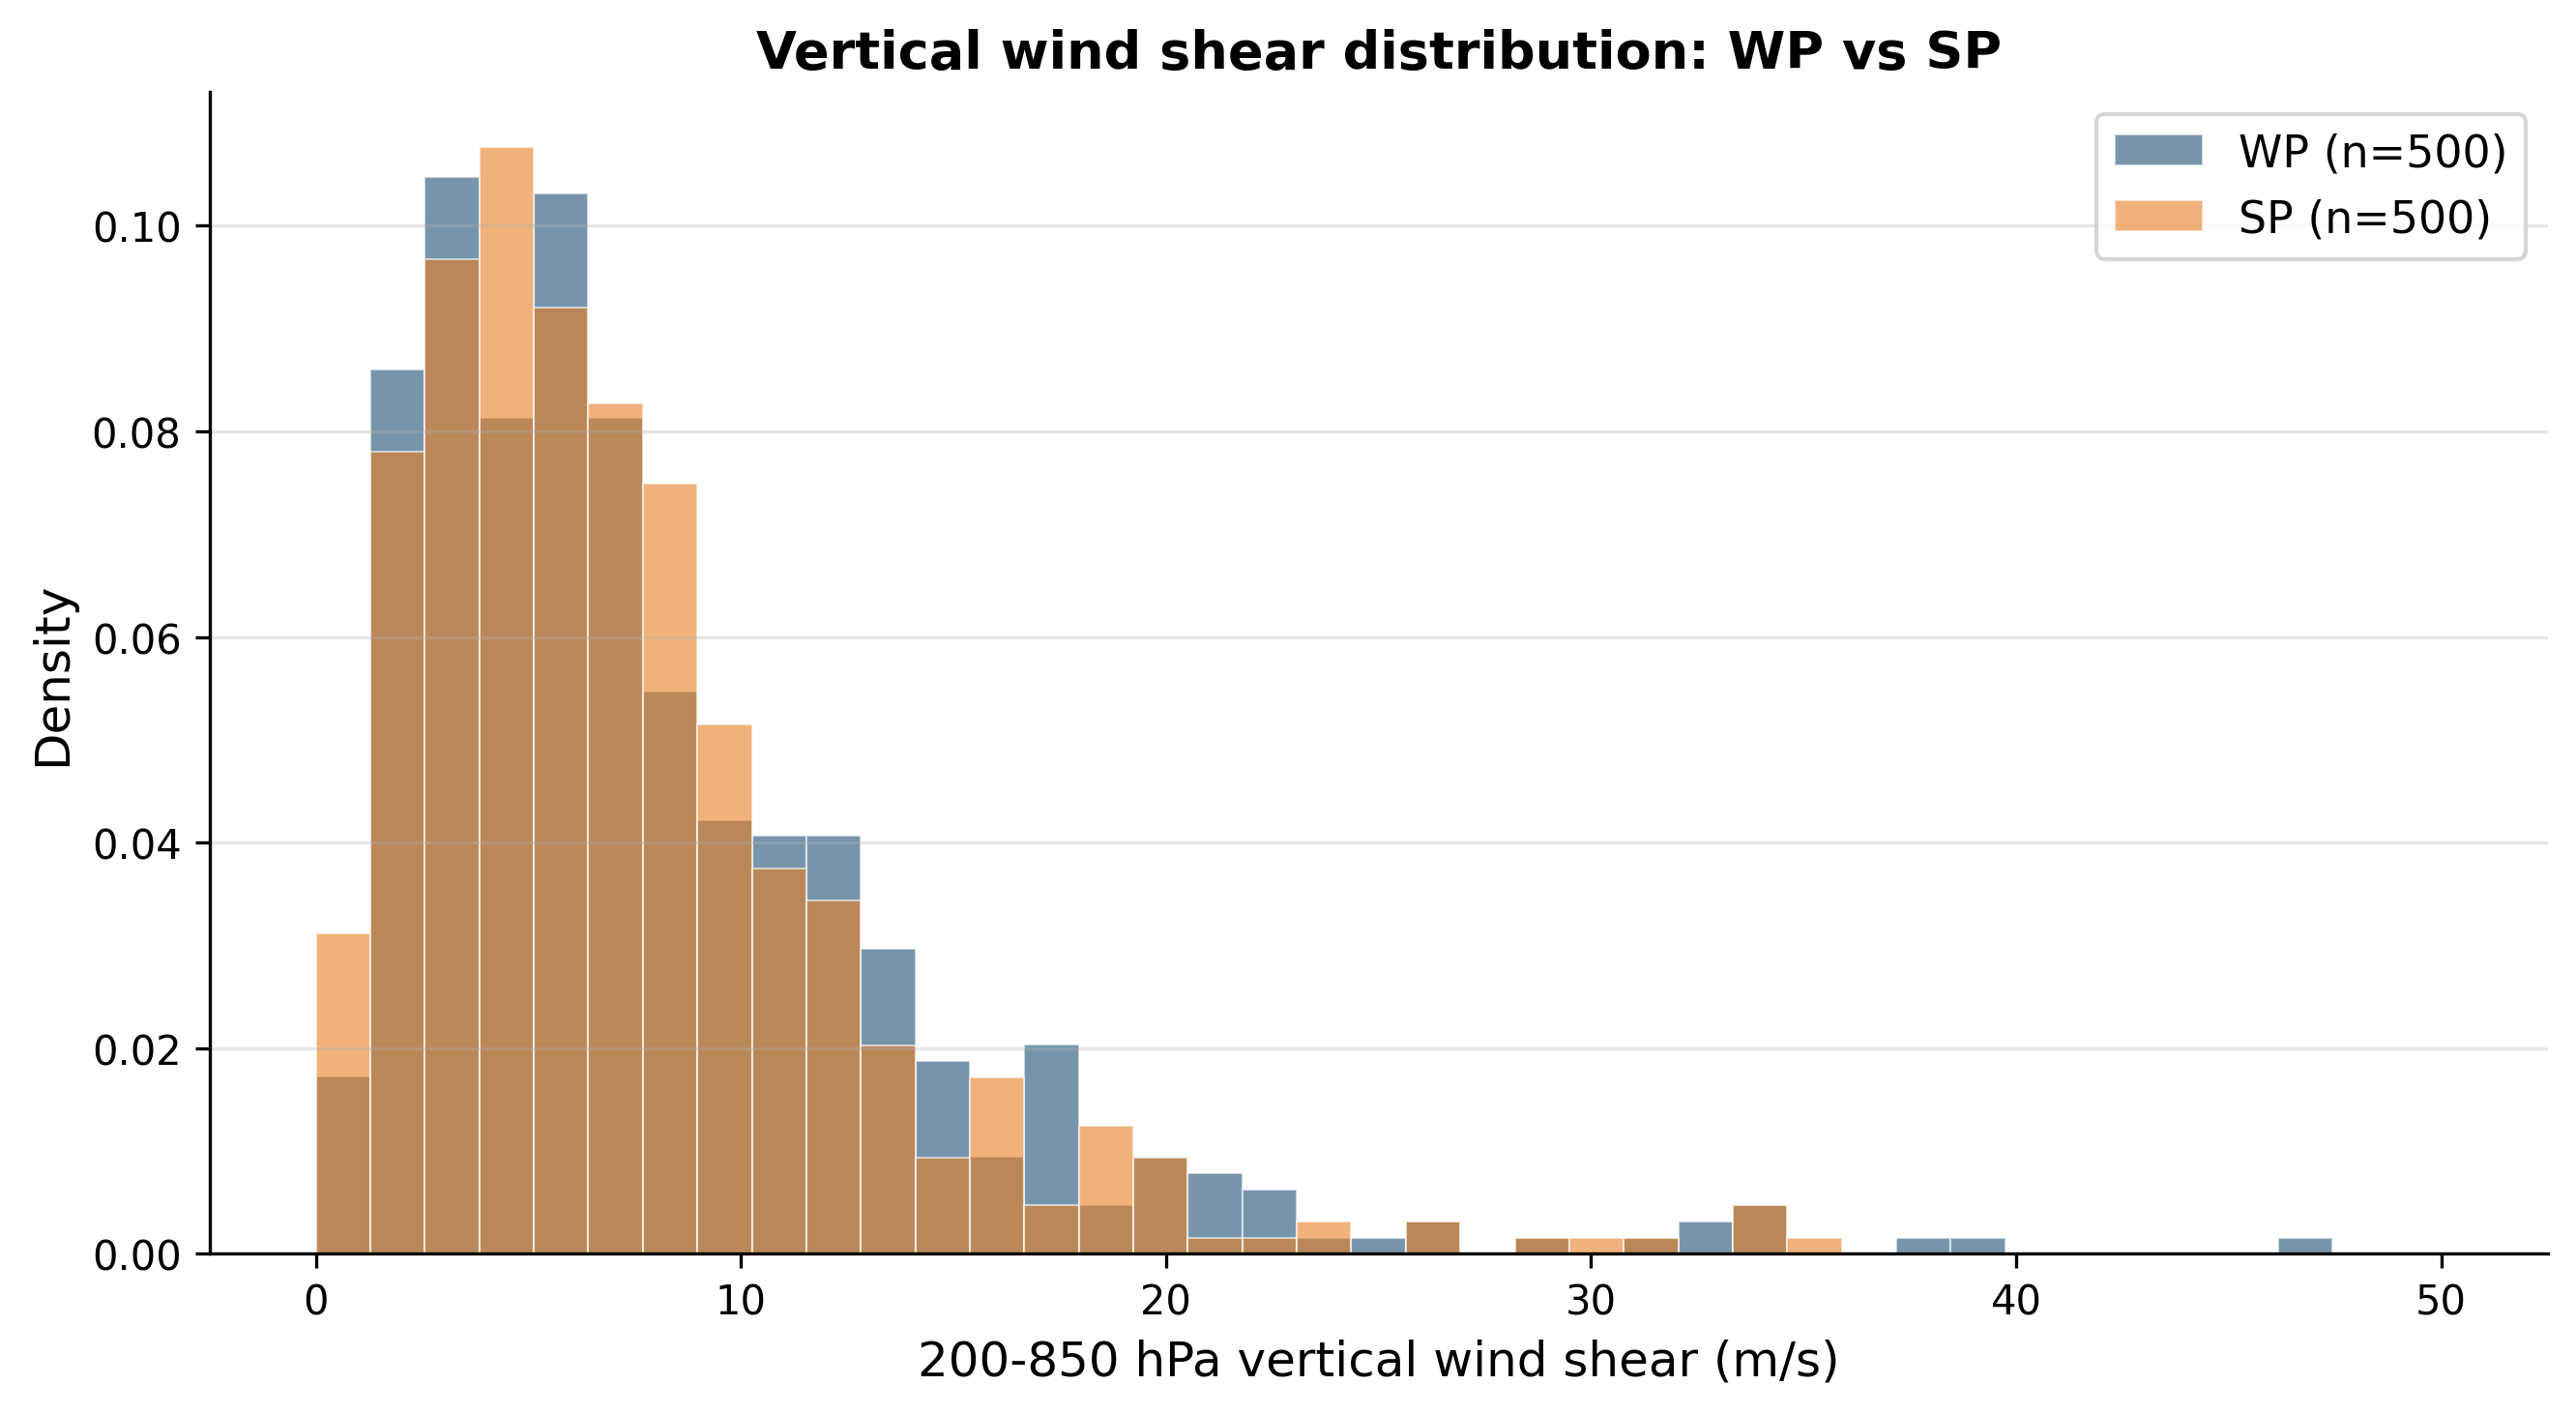
\includegraphics[width=\columnwidth]{../../figures/shear_distribution.png}
{\scriptsize\textbf{Fig.~4:} Vertical wind shear distributions for WP and SP (n=500 each).}

\end{multicols}
% ── References ────────────────────────────────────────────────────
\vspace{4pt}
{\fontsize{6}{7}\selectfont
\textbf{References}\enspace
[1]~Huang et al., \textit{Nat.\ Commun.}, 2025.\enspace
[2]~Qu et al., \textit{npj Clim.\ Atmos.\ Sci.}, 2025.\enspace
[3]~DeMaria \& Kaplan, \textit{Wea.\ and Forecasting}, 1994.\enspace
[4]~Knapp et al., \textit{Bull.\ Amer.\ Meteor.\ Soc.}, 2010.
}
\end{document}
